%%%%%%%%%%%%%%%%%%%%%%%%%%%%%%%%%%%%%%%%%%%%%%%%%%%%%%%%%%%%
%%                     Lösung Aufgabe 2                   %%
%%%%%%%%%%%%%%%%%%%%%%%%%%%%%%%%%%%%%%%%%%%%%%%%%%%%%%%%%%%%

Aus dem gegebenen Spektrum wird die Impulsfolge abgelesen

\begin{align*}
X(f) = j0.1\delta(f+f_3) + j0.15\delta(f+f_2) + j0.25\delta(f+f_1) \\
- j0.1\delta(f-f_3) - j0.15\delta(f-f_2) - j0.25\delta(f-f_1)
\end{align*}

%%%%%%%%%%%%%%%%%%%%%%%%%%%%%%%%%%%%%%%%%%%%%%%%%%%%%%%%%%%%

\subsection{inverse Fouriertransformation} \label{aufg:3a}

Um das Signal zu erhalten, wird eine inverse Fouriertransformation durchgeführt.

\begin{equation*}
x(t) = \int\limits_{-\infty}^{\infty} X(f)e^{j2\pi ft}\mathrm{~d}f \tag{IFT}
\end{equation*}

Für den ersten Term in $X(f)$ wird das Integral ausgewertet. Dieses lässt sich wegen der Abtasteigenschaft der Delta-Distribution (\ref{eq:abtasteigenschaft}) auflösen. Der Exponent wird wegen dem positiven Vorzeichen von $f_3$ negativ.

\begin{align*}
&j0.1 \int\limits_{-\infty}^{\infty} \delta(f+f_3)\cdot e^{j2\pi ft}\mathrm{~d}f = \frac{j0.1}{2\pi} e^{-j2\pi f_3 t} \\
&= j0.1(\cos(2\pi f_3 t)-j\sin(2\pi f_3 t)) = \frac{1}{10} (j\cos(2\pi f_3) + \sin(2\pi f_3))
\end{align*}

\newpage

Die Selbe Rechnung kann nun auf alle Terme angewendet werden. Zu beachten sind dabei die Vorzeichen. Da der Sinus eine gerade Funktion ist, kann das Vorzeichen der Frequenzen herausgezogen werden. Beim Kosinus hat das Vorzeichen im Argument keine Auswirkung.

\begin{align*}
    x(t) &= \frac{1}{10}(j\cos(2\pi f_3 t) +\sin(2\pi f_3 t)) - \frac{1}{10}(j\cos(2\pi f_3 t) -\sin(2\pi f_3 t)) \\
    & + \frac{1.5}{10}(j\cos(2\pi f_2 t) +\sin(2\pi f_2 t)) - \frac{1.5}{10}(j\cos(2\pi f_2 t) -\sin(2\pi f_2 t)) \\
    & + \frac{2.5}{10}(j\cos(2\pi f_1 t) +\sin(2\pi f_1 t)) - \frac{2.5}{10}(j\cos(2\pi f_1 t) -\sin(2\pi f_1 t))
\end{align*}

Die komplexen Kosinusse kürzen sich weg und man erhält

$$ x(t) = \frac{1}{10} (2\sin(2\pi f_3 t) + 3\sin(2\pi f_2 t) + 5\sin(2\pi f_1t)) $$

%%%%%%%%%%%%%%%%%%%%%%%%%%%%%%%%%%%%%%%%%%%%%%%%%%%%%%%%%%%%

\subsection{Abtastung} \label{aufg:3b}

Abtastung: $x[n] := x(nT_s) = x\left(\dfrac{n}{f_s}\right)$

$$
x[n] = \frac{1}{10} \left(5\sin\left(2\pi \frac{f_1}{f_s} t \right) + 3\sin\left(2\pi \frac{f_2}{f_s} t \right) + 2\sin\left(2\pi \frac{f_3}{f_s} t \right) \right)
$$

Für eine schönere Darstellung wird das Signal noch normiert mit $\Omega_n := 2\pi \dfrac{f_n}{f_s} \implies \Omega_s = 2\pi$

$$ 
x[n] = \frac{1}{10} \left(5\sin\left(\Omega_1 t \right) + 3\sin\left( \Omega_2 t \right) + 2\sin\left(\Omega_3 t \right) \right)
$$

In dem Signal kommen nur diskrete Sinusschwingungen vor, welche im Spektrum (Betragsmäßig) zu Delta-Impulsen korrespondieren. Dieses Delta-Impulse treten an den stellen der normierten Kreisfrequenzen $\Omega_1$ bis $\Omega_3$ auf. Das Spektrum ist außerdem periodisch. Es tritt um jedes Vielfaches von $\Omega_S$ das Spektrum erneut auf. (Eigenschaft des abgetasteten Sinus)

\renewcommand{\labelenumi}{(\roman{enumi})}
\begin{enumerate}
\item $f_1 = 400 \mathrm{Hz}$, $f_2 = 800 \mathrm{Hz}$, $f_3 = 1600 \mathrm{Hz}\quad\implies\quad\Omega_1 = \dfrac{1}{5}\pi $, $\Omega_2 = \dfrac{2}{5}\pi $, $\Omega_3 = \dfrac{4}{5}\pi $

Hier befinden sich alle Frequenzen innerhalb der Integrationsgrenzen der inversen DTFT \\ (siehe Tabelle \ref{tab:dtft}). Daher kann das Signal aus diesem Spektrum exakt rekonstruiert werden.

{\centering
\begin{tikzpicture}[x=0.7cm, y=0.4cm, line width=1pt]
 \spectrum;
 {\color{blue}
  \foreach \x/\y/\l in {0.2/5/1, 0.4/3/2, 0.8/2/3} {
      \dirac{\x*pi}{\y}{$\Omega_{\l}$};
      \dirac{-\x*pi}{\y}{$-\Omega_{\l}$};
  }
 }
 {\color{gray}
 \foreach \x/\y in {0.2/5, 0.4/3, 0.8/2} {
    \dirac{2*pi+\x*pi}{\y}{};
    \dirac{2*pi-\x*pi}{\y}{};
    \dirac{-2*pi+\x*pi}{\y}{};
    \dirac{-2*pi-\x*pi}{\y}{};
 }}
\end{tikzpicture}}

\newpage

\item[\label{item:ii}] $f_1 = 2400 \mathrm{Hz}$, $f_2 = 2800 \mathrm{Hz}$, $f_3 = 3600 \mathrm{Hz}\quad\implies\quad\Omega_1 = \dfrac{6}{5}\pi $, $\Omega_2 = \dfrac{7}{5}\pi $, $\Omega_3 = \dfrac{9}{5}\pi $
\label{ii}

Zu beachten ist hier, dass alle $\Omega_n>\pi$ sind. Dieses Kriterium verletzt das Abtasttheorem. Man kann erkennen, dass Aliase der Frequenzen um höhere vielfache der Sampling-Frequenz herunter gespiegelt werden. 

{\centering
 \begin{tikzpicture}[x=0.7cm, y=0.4cm, line width=1pt]
 \spectrum;
 {\color{blue}
  \foreach \x/\y/\l in {0.2/5/1, 0.4/3/2, 0.8/2/3} {
      \dirac{pi+\x*pi}{\y}{$\Omega_{\l}$};
      \dirac{-pi-\x*pi}{\y}{$-\Omega_{\l}$};
  }
 }
 {\color{orange}
  \foreach \x/\y/\l in {0.2/5/1, 0.4/3/2, 0.8/2/3} {
      \dirac{-\x*pi+pi}{\y}{$-\Omega_{\l}^{\prime}$};
      \dirac{\x*pi-pi}{\y}{$\Omega_{\l}^{\prime}$};
  }
}
\draw[decoration={brace, amplitude=5pt, mirror}, decorate] (-pi,-2) -- node[below=2pt] {Aliase} (pi,-2);
\end{tikzpicture}}

Jedoch werden bei der Rekonstruktion des Signals genau diese Aliase wahrgenommen und das Signal lautet daher:

$$ 
x_R[n] = \frac{1}{20\pi} \left(5\sin\left(\Omega'_1 t \right) + 3\sin\left( \Omega'_2 t \right) + 2\sin\left(\Omega'_3 t \right) \right)
$$

mit

$$
\Omega'_1 = \frac{4}{5}\pi,\ \Omega'_2 = \frac{3}{5}\pi,\ \Omega'_3 = \frac{1}{5}\pi \quad\implies\quad f'_1=1600\mathrm{Hz},\ f'_2=1200\mathrm{Hz},\ f'_3=400\mathrm{Hz}
$$ 

Omega mit negativen Vorzeichen sind von oben herab gespiegelt und mit jene mit positiven Vorzeichen von unten hinauf gespiegelt. Die Spiegelachsen sind dabei $\pm\Omega_S$.

\item $f_1 = 4400 \mathrm{Hz}$, $f_2 = 4800 \mathrm{Hz}$, $f_3 = 5600 \mathrm{Hz}\quad\implies\quad\Omega_1 = \dfrac{11}{5}\pi $, $\Omega_2 = \dfrac{12}{5}\pi $, $\Omega_3 = \dfrac{14}{5}\pi $

Hier gilt der gleiche Fall wie in (ii).

{\centering
 \begin{tikzpicture}[x=0.7cm, y=0.4cm, line width=1pt]
 \spectrum;
 {\color{blue}
  \foreach \x/\y/\l in {0.2/5/1, 0.4/3/2, 0.8/2/3} {
      \dirac{2*pi+\x*pi}{\y}{$\Omega_{\l}$};
      \dirac{-2*pi-\x*pi}{\y}{$-\Omega_{\l}$};
  }
 }
 {\color{orange}
  \foreach \x/\y/\l in {0.2/5/1, 0.4/3/2, 0.8/2/3} {
      \dirac{\x*pi}{\y}{$\Omega_{\l}^{\prime}$};
      \dirac{-\x*pi}{\y}{$-\Omega_{\l}^{\prime}$};
  }
}
\draw[decoration={brace, amplitude=5pt, mirror}, decorate] (-pi,-2) -- node[below=2pt] {Aliase} (pi,-2);
\end{tikzpicture}}

Das rekonstruierte Signal ist damit wieder:

$$ 
x_R[n] = \frac{1}{20\pi} \left(5\sin\left(\Omega'_1 t \right) + 3\sin\left( \Omega'_2 t \right) + 2\sin\left(\Omega'_3 t \right) \right)
$$

mit

$$
\Omega'_1 = \frac{1}{5}\pi,\ \Omega'_2 = \frac{2}{5}\pi,\ \Omega'_3 = \frac{4}{5}\pi \quad\implies\quad f'_1=400\mathrm{Hz},\ f'_2=800\mathrm{Hz},\ f'_2=1600\mathrm{Hz}
$$

\end{enumerate}